\PassOptionsToPackage{unicode}{hyperref}
\PassOptionsToPackage{hyphens}{url}
\documentclass{article}
\setcounter{secnumdepth}{6}

\usepackage{amsmath,amssymb}
\usepackage{lmodern}
\usepackage{iftex}
\usepackage[letterpaper, margin=1in, top=0.5in, bottom=1in]{geometry}
\usepackage{listings}
\usepackage{color}
\usepackage{titling}
\usepackage{graphicx}
\usepackage{hyperref}

\ifPDFTeX
  \usepackage[T1]{fontenc}
  \usepackage[utf8]{inputenc}
  \usepackage{textcomp} 
\else 
  \usepackage{unicode-math}
  \defaultfontfeatures{Scale=MatchLowercase}
  \defaultfontfeatures[\rmfamily]{Ligatures=TeX,Scale=1}
\fi
\IfFileExists{upquote.sty}{\usepackage{upquote}}{}
\IfFileExists{microtype.sty}{
  \usepackage[]{microtype}
  \UseMicrotypeSet[protrusion]{basicmath} 
}{}
\makeatletter
\@ifundefined{KOMAClassName}{
  \IfFileExists{parskip.sty}{
    \usepackage{parskip}
  }{
    \setlength{\parindent}{0pt}
    \setlength{\parskip}{6pt plus 2pt 2pt}}
}{
  \KOMAoptions{parskip=half}}
\makeatother
\usepackage{xcolor}
\usepackage{graphicx}

\makeatletter
\def\maxwidth{\ifdim\Gin@nat@width>\linewidth\linewidth\else\Gin@nat@width\fi}
\def\maxheight{\ifdim\Gin@nat@height>\textheight\textheight\else\Gin@nat@height\fi}
\makeatother
\setkeys{Gin}{width=\maxwidth,height=\maxheight,keepaspectratio}
\makeatletter
\def\fps@figure{htbp}
\makeatother
\setlength{\emergencystretch}{3em} 
\providecommand{\tightlist}{
  \setlength{\itemsep}{0pt}\setlength{\parskip}{0pt}}

\ifLuaTeX
  \usepackage{selnolig}  
\fi
\IfFileExists{bookmark.sty}{\usepackage{bookmark}}{\usepackage{hyperref}}
\IfFileExists{xurl.sty}{\usepackage{xurl}}{} 
\urlstyle{same}
\hypersetup{
  hidelinks,
  pdfcreator={LaTeX via pandoc}}

\title{Artifacts - Sprint 6}
\date{}

\begin{document}

\maketitle

\hypertarget{sos-s3} {
\section{Scrum of Scrums}\label{Scrum of Scrums} 
At that time, the team had reorganized to move forward on console, bridge and game Epics.
Mainly the architecture for running the game.jar scripts was updated, client socket communication plus bridge screen communication was implemented, and the functional US of the Pacman game was finalized. Then, in the Lead's Daily a brainstorming session was held to agree on a refactoring of Pacman with the update of the new bridge.jar and also the refactoring of the last script related to the architecture and it was concluded to move forward with the remaining US on the weekend to finish the sprint with half of the estimated points.
}

\href{https://github.com/Pending-Name-21/pac-man/pull/10}{Link: Pacman-Refactor - Pull Request on GitHub}.

\href{https://github.com/Pending-Name-21/miscellany/pull/17}{Link: Refactor-Script - Pull Request on GitHub}.

\href{https://tree.taiga.io/project/joseluis-teran-coffeetime/taskboard/sprint-6-3003}{Link: User Stories of Sprint 6 on Taiga}.

\begin{figure}
\centering
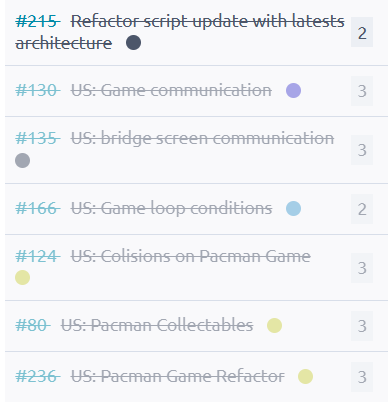
\includegraphics[width=16cm, height=10cm]{./assets/US-Sprint6.png}
\end{figure}

\hypertarget{burndownchart-s3}{
\section{Burn Down Chart}\label{Burn Down Chart S3}}
\href{https://tree.taiga.io/project/joseluis-teran-coffeetime/taskboard/sprint-6-3003}{Link: Sprint 6 Board on Taiga}.

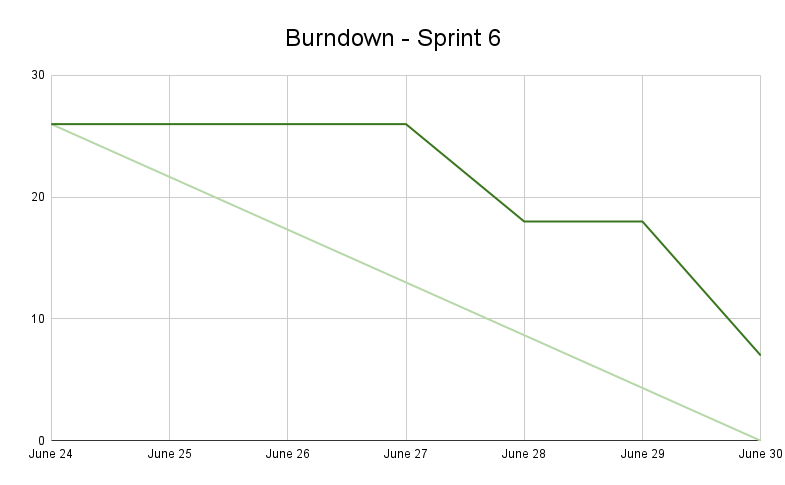
\includegraphics[width=\textwidth]{./assets/Burndown-Sprint6.png}

\hypertarget{startstopcontinueactionitems-s3}{
\section{Start-Stop-Continue-Action Items}\label{Start-Stop-Continue-Action Items S6}}
\href{https://miro.com/app/board/uXjVKDO7l8M=/?moveToWidget=3458764591631763576&cot=14}{Link: Start-Stop-Continue-Action Items Sprint 6 on Miro}.

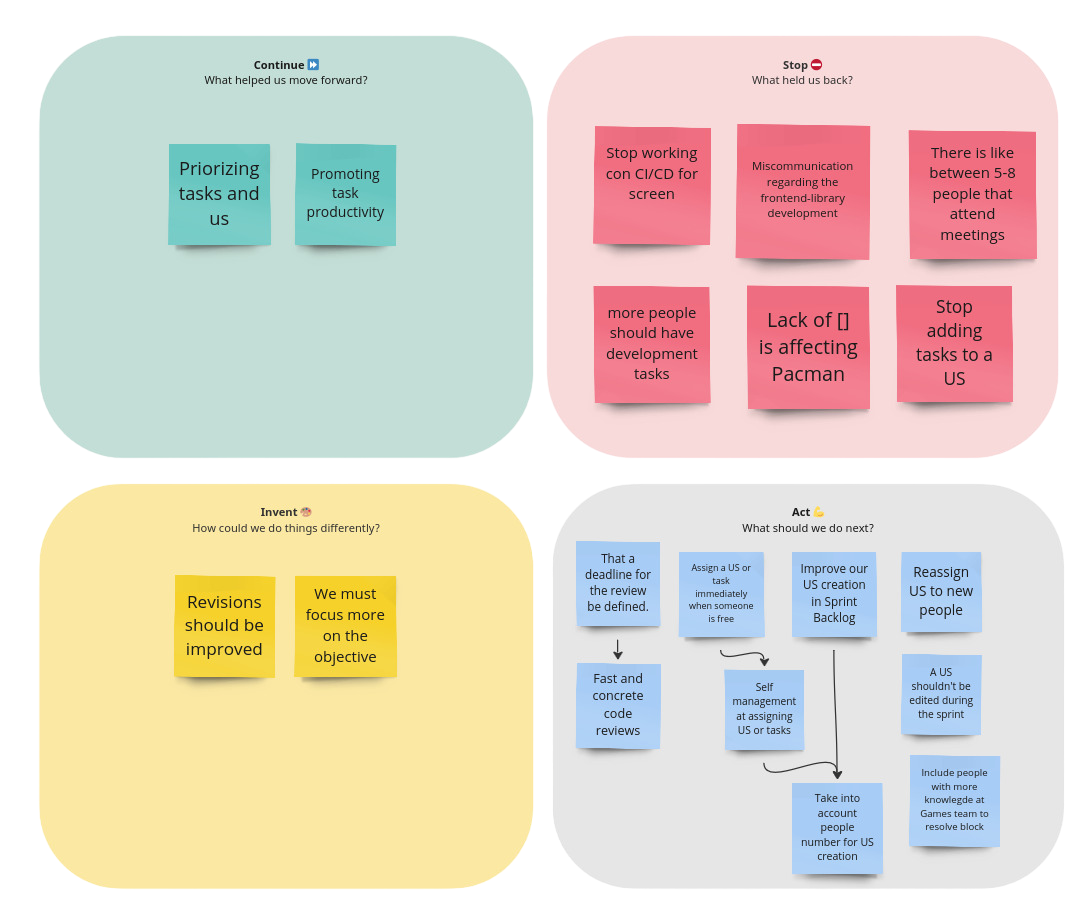
\includegraphics[width=\textwidth]{./assets/retrospective-s6.png}

\end{document}
